\documentclass[9pt]{article}
\usepackage{amsmath,amsthm,amscd,amssymb,mathrsfs,tikz}
\usepackage{latexsym,epsf,epsfig}
\usepackage{sectsty}
\usepackage{hyperref}
\usepackage{graphicx}
\usepackage{booktabs, multirow} % for borders and merged ranges
\usepackage{soul}% for underlines
\usepackage{xcolor,colortbl} % for cell colors
\usepackage{changepage,threeparttable} % for wide tables
\usepackage[left=1.2in, right=1.2in, top=1in, bottom=1in]{geometry} %The above set the parameters adjust the margins. There are many ways to do this, and frankly, what is above is not the best. However, it will work the time being.

\newcommand{\ds}{\displaystyle}
\newcommand{\sU}{\mathscr U}
% Theorem
\theoremstyle{plain}
\newtheorem{theorem}{Theorem}
% Margins
\topmargin=-0.45in
\evensidemargin=0in
\oddsidemargin=0in
\textwidth=6.5in
\textheight=9.0in
\headsep=0.25in

\title{ MATH 341: Homework 4}
\author{ Aren Vista }

\begin{document}
\maketitle
\section{Question 1}
\begin{center}
	What lower triangular matrix $E$ puts $A$ into upper triangular form $EA=U$? \\
	Multiply by $E^{-1}=L$ to factor $A$ into $LU$:
\end{center}
\[
	A =
	\begin{bmatrix}
		2 & 1 & 0 \\
		0 & 4 & 2 \\
		6 & 3 & 5
	\end{bmatrix}
\]
\[
	\underbrace{\begin{bmatrix}
			2 & 1 & 0 \\
			0 & 4 & 2 \\
			6 & 3 & 5
		\end{bmatrix}}_{A}
	\xrightarrow{R_3 = R_3 - 3R_1}
	\underbrace{\begin{bmatrix}
			2 & 1 & 0 \\
			0 & 4 & 2 \\
			0 & 0 & 5
		\end{bmatrix}}_{U}
	\implies
	\underbrace{\begin{bmatrix}
			1  & 0 & 0 \\
			0  & 1 & 0 \\
			-3 & 0 & 1 \\
		\end{bmatrix}}_{E}
\]
\[
	\underbrace{\begin{bmatrix}
			1  & 0 & 0 \\
			0  & 1 & 0 \\
			-3 & 0 & 1 \\
		\end{bmatrix}}_{E}
	\xrightarrow{\text{Multiply off-diag $-1$}}
	\underbrace{\begin{bmatrix}
			1 & 0 & 0 \\
			0 & 1 & 0 \\
			3 & 0 & 1 \\
		\end{bmatrix}}_{L}
\]

\[
	\begin{gathered}
		\begin{bmatrix}
			2 & 1 & 0 \\
			0 & 4 & 2 \\
			6 & 3 & 5
		\end{bmatrix}
		=
		\begin{bmatrix}
			1 & 0 & 0 \\
			0 & 1 & 0 \\
			3 & 0 & 1 \\
		\end{bmatrix}
		\begin{bmatrix}
			2 & 1 & 0 \\
			0 & 4 & 2 \\
			0 & 0 & 5
		\end{bmatrix} \\ \\
		A = LU
	\end{gathered}
\]

\section{Question 2}
\begin{center}
	This problem shows how the one-step inverses multiply to give $L$.
	You see this best when $A = L$ is already lower triangular with $1$'s on the diagonal. Then $U=I$
\end{center}
\[
	A =
	\begin{bmatrix}
		1 & 0 & 0 \\
		a & 1 & 0 \\
		b & c & 1
	\end{bmatrix} \quad\quad
	E_1 =
	\begin{bmatrix}
		1  & 0 & 0 \\
		-a & 1 & 0 \\
		-b & 0 & 1
	\end{bmatrix} \quad\quad
	E_2 =
	\begin{bmatrix}
		1 & 0  & 0 \\
		0 & 1  & 0 \\
		0 & -c & 1
	\end{bmatrix}
\]
\begin{itemize}
	\item  1) $E_2E_2$ to find $EA=I$
	\item  2) $E_1^{-1}E_2^{-1}$ to find $A=L$
	\item  3) The multipliers $a,b,c$ are mixed up in $E = L^{-1}$ but are perfect in $L$
\end{itemize}

\subsection{P.1}
\[
	\begin{bmatrix}
		1  & 0 & 0 \\
		-a & 1 & 0 \\
		-b & 0 & 1
	\end{bmatrix}
	\begin{bmatrix}
		1 & 0  & 0 \\
		0 & 1  & 0 \\
		0 & -c & 1
	\end{bmatrix}
	=
	\underbrace{
		\begin{bmatrix}
			1  & 0  & 0 \\
			-a & 1  & 0 \\
			-b & -c & 1
		\end{bmatrix}}_{E_1E_2}
\]  \\
\[
	\begin{bmatrix}
		1  & 0  & 0 \\
		-a & 1  & 0 \\
		-b & -c & 1
	\end{bmatrix}
	\begin{bmatrix}
		1 & 0 & 0 \\
		a & 1 & 0 \\
		b & c & 1
	\end{bmatrix}  =
	\begin{bmatrix}
		1 & 0 & 0 \\
		0 & 1 & 0 \\
		0 & 0 & 1
	\end{bmatrix}

\]

\subsection{P.2}
\[
	E_1^{-1} =
	\begin{bmatrix}
		1 & 0 & 0 \\
		a & 1 & 0 \\
		b & 0 & 1
	\end{bmatrix} \quad\quad
	E_2^{-1} =
	\begin{bmatrix}
		1 & 0 & 0 \\
		0 & 1 & 0 \\
		0 & c & 1
	\end{bmatrix}  \quad\quad
	E_1^{-1}E_2^{-1} =
	\begin{bmatrix}
		1 & 0 & 0 \\
		a & 1 & 0 \\
		b & c & 1
	\end{bmatrix} = L
\]



\section{Question 3}
\begin{center}Compute $L,U$ for the matrix $A$: \end{center}
\[
	A =
	\begin{bmatrix}
		a & a & a & a \\
		a & b & b & b \\
		a & b & c & c \\
		a & b & c & d
	\end{bmatrix}
\]
\begin{center} Find four condition on $a,b,c,d$ to get $A = LU$ with four non-zero pivots. \end{center}

\section{Question 4}
\[
	\begin{gathered}
		\text{What multiple of $a$ should be substraced from $b$ to make the resut $A_2$ orthogonal to $a$? Sketch a figure to show $a,b,A_2$} \\
		a = \begin{bmatrix} 1 \\ 1 \end{bmatrix} \quad\quad b = \begin{bmatrix} 4 \\ 0 \end{bmatrix} \\
	\end{gathered}
\]
\[
	\begin{gathered}
		\exists~ A_2         =  b-xa \ni A_2 \perp a                                           \\
		\implies a \cdot A_2 =  0  = a \cdot (b-xa) =  0 ab-xaa =  0                           \\
		\implies x           =  \frac{ab}{aa} = \frac{(1 \times 4) + (0)}{2} = \frac{4}{2} = 2 \\
		A_2                  =  b -2a = \begin{bmatrix} 2 \\ -2 \end{bmatrix}
	\end{gathered}
\]
\begin{center}
	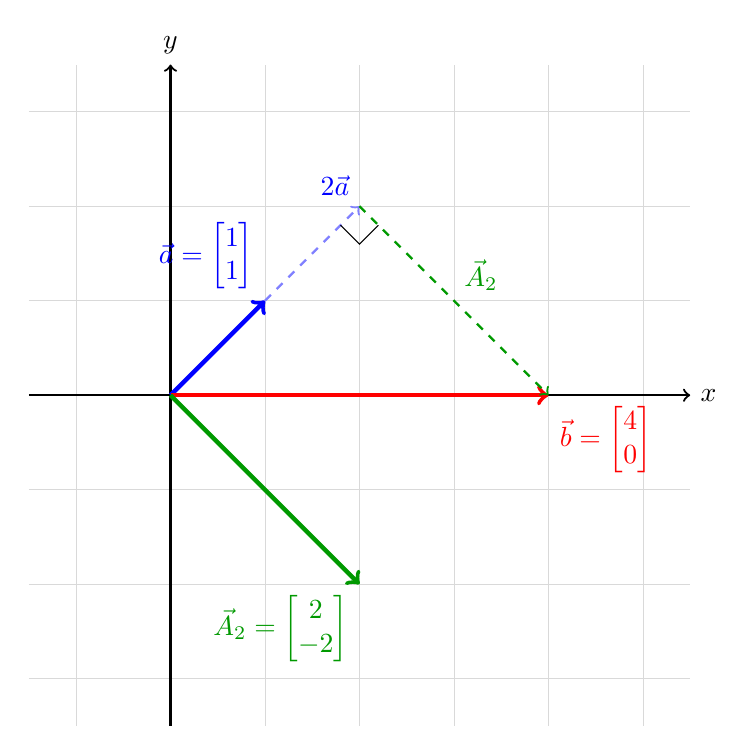
\begin{tikzpicture}[scale=1.2]
		% Grid and Axes
		\draw[very thin,color=gray!30,step=1.0] (-1.5,-3.5) grid (5.5,3.5);
		\draw[->,thick] (-1.5,0) -- (5.5,0) node[right] {$x$};
		\draw[->,thick] (0,-3.5) -- (0,3.5) node[above] {$y$};

		% Vector a
		\draw[->, ultra thick, blue] (0,0) -- (1,1) node[above left] {$\vec{a} = \begin{bmatrix} 1 \\ 1 \end{bmatrix}$};

		% Vector 2a (projection of b onto a)
		\draw[->, thick, blue!50, dashed] (1,1) -- (2,2) node[above left, text=blue] {$2\vec{a}$};

		% Vector b
		\draw[->, ultra thick, red] (0,0) -- (4,0) node[below right] {$\vec{b} = \begin{bmatrix} 4 \\ 0 \end{bmatrix}$};

		% Vector A_2 from origin
		\draw[->, ultra thick, green!60!black] (0,0) -- (2,-2) node[below left] {$\vec{A}_2 = \begin{bmatrix} 2 \\ -2 \end{bmatrix}$};

		% Vector A_2 translated to form the orthogonal triangle (b - 2a)
		\draw[->, thick, green!60!black, dashed] (2,2) -- (4,0) node[midway, above right] {$\vec{A}_2$};

		% Right angle symbol at the projection point (2,2)
		\draw (1.8,1.8) -- (2.0,1.6) -- (2.2,1.8);

	\end{tikzpicture}
\end{center}

\section{Question 5}
\begin{center} Complete the Gram-Schmidt process in the prior problem via computing \end{center}
\[
	a_1 = \frac{a}{\left\| a \right\|} \quad\quad \\
	A_2 = b - (b^Tq_1)q_1 \quad\quad \\
	q_2 = \frac{A_2}{\left\| A_2 \right\|} \quad\quad
\]
\[
    a = 
    \begin{bmatrix}
        1 \\ 1
    \end{bmatrix}
    b = 
    \begin{bmatrix}
        4 \\ 0
    \end{bmatrix}
    A_2 = 
    \begin{bmatrix}
        2 \\ -2
    \end{bmatrix}
\] 


\end{document}
